\documentclass{article}
\usepackage[utf8]{inputenc}
\usepackage{graphicx}
\title{PS6_Kontchou}
\author{kevin.kontchou }
\date{March 2018}

\begin{document}

\maketitle

\section{Data Cleaning Process}
{I used data from my PS5 assignment as well as found some new data on GDP growth percentage in Cameroon over a period of 20 years. I deleted the categories of data that had too many NAs like electrical consumption. I reformatted some of the data that I scraped from the web from French style numeric formatting with commas instead of decimal points to the standard style. I also removed the top empty row of data. I added a titles and named the axes for each of my graphs.}

\textbf{}

\section{GDP Growth Graph}
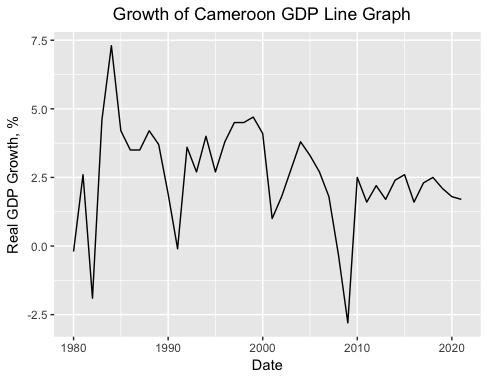
\includegraphics[height = 6cm width = 7cm]{RplotCamLineGraph}
\textbf{this graph illustrates the GDP growth rate as a percentage in Cameroon. The graph helps illustrate the volatility of GDP growth rate percentage of Cameroon. As you can see the growth rate took a hit during the global recession in 2008. So although most of Africa did not necessarily play a large role in the global economic system, countries like Cameroon still felt the effects.}

\section{Fertility Graph}
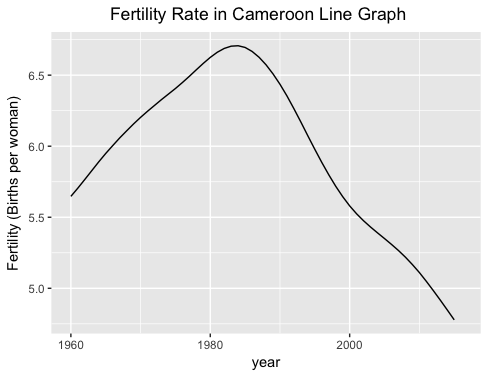
\includegraphics[height = 6cm width = 7cm]{RplotCamFertility}
{This graph helps illustrate the decline in fertility rate that has been occurring in Cameroon. The graph shows the fertility rate started to decline in 1980s, which can be attributed to several factors including the reaction to the spread of HIV/AIDs in west Africa during the 80s.}

\section{Life Expectancy Graph}
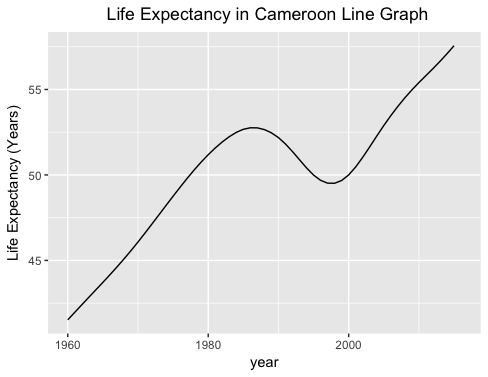
\includegraphics[height = 6cm width = 7cm]{RplotCamLifeExpect}
{This graph illustrates the overall increase in life expectancy that is expected to happen when an economy is developing and the overall GDP is rising. The dip during the early 1980s to mid 1990s can also be attributed partly to the spread of the HIV/AIDs epidemic. The prevelance of HIV drugs was not yet available in Cameroon until late 1990s and 2000s.}
\end{document}
